\subsection{ソフトウェア設計戦略と方法}

設計戦略と方法は、設計プロセスを進めるための考え方である。方法によって、何を最初に見るか、どのように分解するか、どの概念を中心に置くかが異なる。

\subsubsection{一般戦略}

一般的な設計戦略には、分割統治、段階的詳細化、トップダウン、ボトムアップ、反復、増分、パターン利用などがある。

\term{分割統治}{divide and conquer} は、大きな問題を小さな問題に分けて解く考え方である。\term{段階的詳細化}{stepwise refinement} は、粗い設計から始め、徐々に詳細を追加する考え方である。トップダウンは全体から部分へ進む。ボトムアップは既存部品や低水準機能から全体を組み立てる。

実務では、これらは単独で使われるというより、組み合わせて使われる。最初にトップダウンで全体構造を作り、既存部品をボトムアップで組み込み、反復しながら詳細化することが多い。

\subsubsection{機能指向・構造化設計}

\term{機能指向設計}{Function-Oriented Design} または\term{構造化設計}{Structured Design} は、ソフトウェアの主要機能を見つけ、それを上位から下位へ分解する古典的な方法である。

この方法では、データフロー図や処理記述を使い、入力がどの処理を通って出力へ変換されるかを考える。業務処理の流れが明確で、機能分解しやすいシステムで理解しやすい。一方、状態やデータ構造、イベント、オブジェクト間の相互作用が複雑な場合は、別の方法と組み合わせる必要がある。

\subsubsection{データ中心設計}

\term{データ中心設計}{Data-Centered Design} は、プログラムが扱うデータ構造から設計を始める方法である。入力データ構造と出力データ構造を明らかにし、入力を出力へ変換する処理単位を設計する。

データが安定しており、処理がデータ構造に強く依存する場合に有効である。たとえば、ファイル変換、帳票生成、データ処理パイプラインなどでは、データ構造を中心に考えると設計しやすい。

\subsubsection{オブジェクト指向設計}

\term{オブジェクト指向設計}{Object-Oriented Design} は、オブジェクトを中心に設計する方法である。オブジェクトは、データと操作を一体として持つ概念である。設計では、クラス、属性、メソッド、関連、継承、多態性、責務を考える。

初期のオブジェクト指向設計では、名詞からオブジェクトを見つけ、動詞からメソッドを見つける方法が使われた。現在では、単に名詞を拾うだけでなく、責務を中心に設計する考え方が重要である。クラスが何を知り、何を行い、誰と協調するかを考える。

SOLID原則は、クラス設計でよく参照される考え方である。単一責任、開放閉鎖、リスコフ置換、インタフェース分離、依存関係逆転の頭文字である。これらは、変更しやすく理解しやすいオブジェクト指向設計を目指すための指針である。

\subsubsection{利用者中心設計}

\term{利用者中心設計}{User-Centered Design} は、利用者とその作業、目的、文脈を深く理解したうえで設計する方法である。単に画面をきれいにすることではなく、利用者が何を達成したいか、どのような環境で使うか、どのような誤りを起こしやすいかを考える。

利用者中心設計では、利用者要求の収集、作業の流れの整理、プロトタイプやモックアップの作成、利用者評価を行う。使いやすさが重要なシステムでは、利用者中心設計を後から追加するのではなく、設計の初期から組み込む必要がある。

\subsubsection{構成要素ベース設計}

\term{構成要素ベース設計}{Component-Based Design, CBD} は、独立して配置・利用できる構成要素を組み合わせてシステムを作る方法である。各構成要素は、明確なインタフェースと依存関係を持つ。

この方法の目的は、再利用、独立開発、交換容易性、統合容易性を高めることである。構成要素ベース設計では、共通API、サービスごとのAPI、部品のバージョン、依存関係、配置方法が重要になる。

\subsubsection{イベント駆動設計}

\term{イベント駆動設計}{Event-Driven Design} は、イベントに反応して処理を行う設計方法である。イベントとは、利用者操作、メッセージ受信、状態変化、タイマー発火、センサー入力などである。

イベント駆動設計では、発行・購読方式がよく使われる。送信側はイベントを発行し、受信側は関心のあるイベントを購読する。これにより、送信側と受信側の結合を弱められる。大規模で拡張性が必要なシステムでは有効だが、イベントの順序、重複、遅延、失敗時の影響を慎重に設計する必要がある。

\subsubsection{アスペクト指向設計}

\term{アスペクト指向設計}{Aspect-Oriented Design, AOD} は、横断的関心事をアスペクトとして分離する方法である。横断的関心事とは、ログ、セキュリティ確認、トランザクション、例外処理など、複数の機能にまたがる関心である。

アスペクト指向の考え方は、必ずしも独立した設計手法として広く使われているわけではない。しかし、アプリケーションフレームワークやライブラリでは、宣言や設定によって横断的な振る舞いを追加する形で利用されることがある。

\subsubsection{制約に基づく設計}

\term{制約に基づく設計}{Constraint-Based Design} は、制約を使って設計空間を狭める方法である。設計空間とは、可能な設計案全体の集合である。制約は、不可能または受け入れられない案を除外する役割を持つ。

制約には、ハードウェア、ソフトウェア、データ、操作手順、インタフェース、法令、性能、費用、納期などが含まれる。制約を明確にすれば、設計探索が速くなる。一方、制約が多すぎる場合や互いに矛盾する場合は、解が見つからないこともある。

\subsubsection{ドメイン駆動設計}

\term{ドメイン駆動設計}{Domain-Driven Design} は、対象領域の概念と言葉を中心に設計する方法である。ここでいうドメインとは、銀行、医療、物流、教育、ゲームなど、ソフトウェアが扱う問題領域である。

ドメイン駆動設計では、分析者、設計者、開発者、業務専門家が共有する言葉を重視する。この共有語彙を使って、オブジェクト、役割、イベント、活動、規則を設計記述に反映する。言葉がずれると、実装もずれるため、ドメインの語彙を設計の中心に置くことが重要である。

\subsubsection{その他の方法}

その他にも、多くの設計方法がある。反復型・適応型の方法では、厳密な要求と設計を最初にすべて固定するのではなく、ソフトウェア増分を作りながら設計を調整する。

\term{サービス指向設計}{Service-Oriented Design} は、分散されたサービスを組み合わせてソフトウェアを作る方法である。HTTP、HTTPS、SOAPなどの標準プロトコルを使い、異なる提供者のサービスをつなぐことがある。

\par\smallskip
\begin{center}
\centering
\IfFileExists{assets/generated_figures/ch03/fig-ch03-10.png}{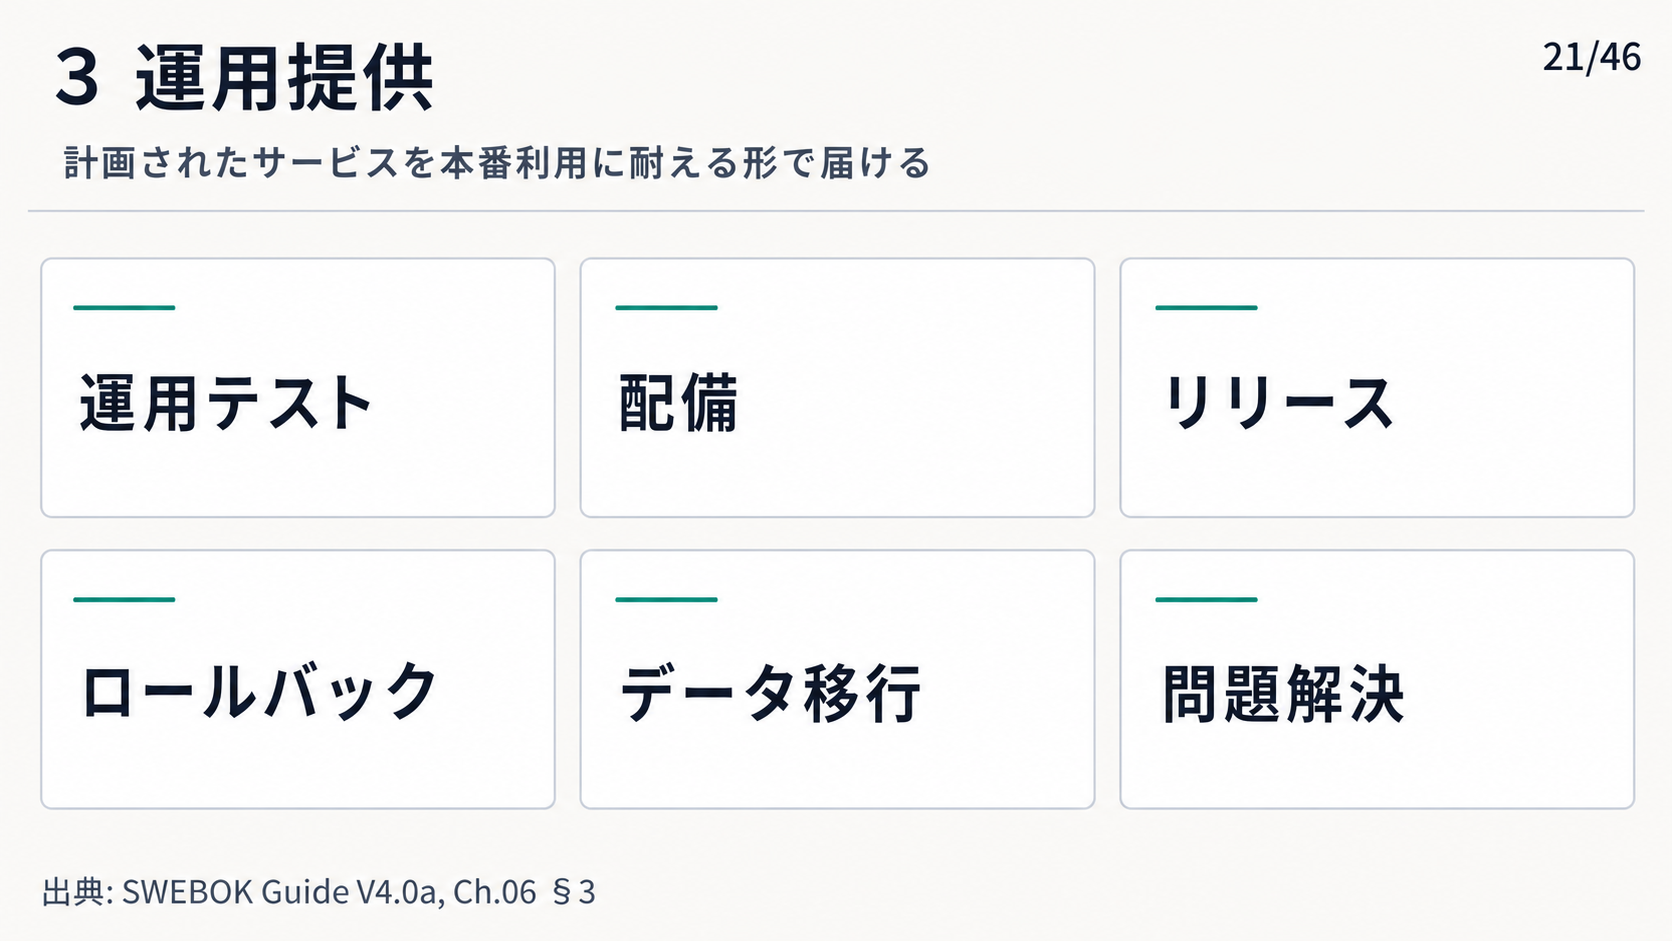
\includegraphics[width=0.96\linewidth]{assets/generated_figures/ch03/fig-ch03-10.png}}{\fbox{\parbox[c][48mm][c]{0.9\linewidth}{\centering 画像生成待ち\\設計戦略と中心概念の対応図}}}
\par\smallskip
\refstepcounter{figure}\label{fig:ch03-10}図 \thefigure: 設計戦略と中心概念の対応図
\end{center}
図 \thefigure は、設計戦略と中心概念の対応図を視覚的に整理したものである。
\par\smallskip
